\documentclass[11pt]{article}
\usepackage[a4paper,margin=25mm]{geometry}
\usepackage[T1]{fontenc}
\usepackage{lmodern,microtype}
\usepackage{amsmath,amssymb}
\usepackage{booktabs,tabularx,longtable,array}
\usepackage{graphicx,tikz}
\usepackage{flafter}
\usetikzlibrary{arrows.meta,positioning}
\usepackage{enumitem}
\usepackage[numbers,sort&compress]{natbib}
\usepackage{xcolor}
\definecolor{navy}{HTML}{153449}
\definecolor{teal}{HTML}{087D8B}
\usepackage{hyperref}
\usepackage{xurl}
\hypersetup{colorlinks=true,linkcolor=navy,citecolor=teal,urlcolor=teal}
\usepackage{fancyhdr}
\pagestyle{fancy}
\fancyhf{}
\fancyhead[L]{\small Warrant: evaluation and evidence}
\fancyhead[R]{\small Technical preprint}
\fancyfoot[C]{\thepage}
\setlength{\headheight}{14pt}
\setlength{\parskip}{4pt}
\setlength{\parindent}{0pt}
\setlength{\emergencystretch}{2em}
\setlist{nosep,leftmargin=*}
% Generated from paper/metadata.json.
\newcommand{\PaperAuthor}{Aditya Singh}
\newcommand{\PaperTitle}{Warrant: Reproducible Evaluation and Evidence Management for AI Detectors}
\newcommand{\PaperAffiliation}{IIT Kharagpur}
\newcommand{\PaperDate}{05 November 2026}
\newcommand{\PaperVersion}{1.0}
\newcommand{\PaperRepository}{https://github.com/Aditya26189/Warrant}
\newcommand{\PaperRepositoryRef}{warrant-preprint-v1.0}

% Generated from retained evidence; original results are unchanged.
\expandafter\def\csname claimC001\endcsname{0.8256}
\expandafter\def\csname ciC001\endcsname{[0.7934, 0.8567]}
\expandafter\def\csname claimC002\endcsname{0.0794}
\expandafter\def\csname ciC002\endcsname{[0.0496, 0.1115]}
\expandafter\def\csname claimC003\endcsname{0.8800}
\expandafter\def\csname ciC003\endcsname{[0.7500, 1.0000]}
\expandafter\def\csname claimC004\endcsname{0.0417}
\expandafter\def\csname ciC004\endcsname{[0.0267, 0.0583]}
\expandafter\def\csname claimC005\endcsname{0.4617}
\expandafter\def\csname ciC005\endcsname{-}
\expandafter\def\csname claimC006\endcsname{0.8256}
\expandafter\def\csname ciC006\endcsname{-}
\expandafter\def\csname claimC007\endcsname{A}
\expandafter\def\csname ciC007\endcsname{-}
\expandafter\def\csname claimC008\endcsname{-0.0110}
\expandafter\def\csname ciC008\endcsname{[-0.0200, -0.0026]}
\expandafter\def\csname claimC009\endcsname{1.5922}
\expandafter\def\csname ciC009\endcsname{-}
\expandafter\def\csname claimC010\endcsname{0.20}
\expandafter\def\csname ciC010\endcsname{-}
\expandafter\def\csname claimC011\endcsname{0.6462}
\expandafter\def\csname ciC011\endcsname{[0.5950, 0.7051]}
\expandafter\def\csname claimC012\endcsname{0.7749}
\expandafter\def\csname ciC012\endcsname{[0.7227, 0.8290]}
\expandafter\def\csname claimC013\endcsname{1.678}
\expandafter\def\csname ciC013\endcsname{[1.545, 1.831]}
\expandafter\def\csname claimC014\endcsname{0.6209}
\expandafter\def\csname ciC014\endcsname{[0.5667, 0.6815]}
\expandafter\def\csname claimC015\endcsname{0.7679}
\expandafter\def\csname ciC015\endcsname{[0.7137, 0.8214]}
\expandafter\def\csname claimC016\endcsname{0.6318}
\expandafter\def\csname ciC016\endcsname{[0.5782, 0.6880]}
\expandafter\def\csname claimC017\endcsname{0.7743}
\expandafter\def\csname ciC017\endcsname{[0.7220, 0.8281]}
\expandafter\def\csname claimC018\endcsname{1.677}
\expandafter\def\csname ciC018\endcsname{[1.535, 1.826]}
\expandafter\def\csname claimC019\endcsname{True}
\expandafter\def\csname ciC019\endcsname{-}
\expandafter\def\csname claimC020\endcsname{0.2171}
\expandafter\def\csname ciC020\endcsname{[0.1800, 0.2564]}
\expandafter\def\csname claimC021\endcsname{0.1062}
\expandafter\def\csname ciC021\endcsname{[0.0885, 0.1260]}
\expandafter\def\csname claimC022\endcsname{0.9216}
\expandafter\def\csname ciC022\endcsname{[0.8676, 0.9684]}
\expandafter\def\csname claimC023\endcsname{0.3603}
\expandafter\def\csname ciC023\endcsname{[0.3173, 0.4063]}
\expandafter\def\csname claimC024\endcsname{0.1865}
\expandafter\def\csname ciC024\endcsname{[0.1635, 0.2125]}
\expandafter\def\csname claimC025\endcsname{0.8715}
\expandafter\def\csname ciC025\endcsname{[0.8218, 0.9214]}
\expandafter\def\csname claimC026\endcsname{0.7367}
\expandafter\def\csname ciC026\endcsname{[0.6974, 0.7783]}
\expandafter\def\csname claimC027\endcsname{0.4677}
\expandafter\def\csname ciC027\endcsname{[0.4365, 0.4990]}
\expandafter\def\csname claimC028\endcsname{0.7105}
\expandafter\def\csname ciC028\endcsname{[0.6690, 0.7506]}
\expandafter\def\csname claimC029\endcsname{0.8135}
\expandafter\def\csname ciC029\endcsname{[0.7797, 0.8447]}
\expandafter\def\csname claimC030\endcsname{0.5015}
\expandafter\def\csname ciC030\endcsname{[0.4546, 0.5479]}
\expandafter\def\csname claimC031\endcsname{0.5553}
\expandafter\def\csname ciC031\endcsname{[0.5105, 0.6015]}
\expandafter\def\csname claimC032\endcsname{0.5433}
\expandafter\def\csname ciC032\endcsname{[0.5050, 0.5833]}
\expandafter\def\csname claimC033\endcsname{401}
\expandafter\def\csname ciC033\endcsname{-}
\expandafter\def\csname claimC034\endcsname{450}
\expandafter\def\csname ciC034\endcsname{-}
\expandafter\def\csname claimC035\endcsname{0.3526}
\expandafter\def\csname ciC035\endcsname{-}
\expandafter\def\csname claimC036\endcsname{0.0543}
\expandafter\def\csname ciC036\endcsname{-}
\expandafter\def\csname claimC037\endcsname{13}
\expandafter\def\csname ciC037\endcsname{-}
\expandafter\def\csname claimC038\endcsname{4}
\expandafter\def\csname ciC038\endcsname{-}
\expandafter\def\csname claimC039\endcsname{39}
\expandafter\def\csname ciC039\endcsname{-}
\expandafter\def\csname claimC040\endcsname{0.1176}
\expandafter\def\csname ciC040\endcsname{[0.0500, 0.2000]}
\expandafter\def\csname claimC041\endcsname{0.5455}
\expandafter\def\csname ciC041\endcsname{[0.2592, 0.9002]}
\expandafter\def\csname claimC042\endcsname{0.2843}
\expandafter\def\csname ciC042\endcsname{[0.2075, 0.3810]}
\expandafter\def\csname claimC043\endcsname{0.7436}
\expandafter\def\csname ciC043\endcsname{[0.5416, 0.9584]}
\expandafter\def\csname claimC044\endcsname{0.6176}
\expandafter\def\csname ciC044\endcsname{[0.5185, 0.7128]}
\expandafter\def\csname claimC045\endcsname{0.8630}
\expandafter\def\csname ciC045\endcsname{[0.7262, 0.9828]}
\expandafter\def\csname claimC046\endcsname{0.7941}
\expandafter\def\csname ciC046\endcsname{[0.6981, 0.8846]}
\expandafter\def\csname claimC047\endcsname{0.6532}
\expandafter\def\csname ciC047\endcsname{[0.5114, 0.8100]}
\expandafter\def\csname claimC048\endcsname{0.1471}
\expandafter\def\csname ciC048\endcsname{[0.0714, 0.2341]}
\expandafter\def\csname claimC049\endcsname{0.5357}
\expandafter\def\csname ciC049\endcsname{[0.2812, 0.8621]}
\expandafter\def\csname claimC050\endcsname{0.0000}
\expandafter\def\csname ciC050\endcsname{[0.0000, 0.0183]}
\expandafter\def\csname claimC051\endcsname{0.4221}
\expandafter\def\csname ciC051\endcsname{-}
\expandafter\def\csname claimC052\endcsname{0.3900}
\expandafter\def\csname ciC052\endcsname{-}
\expandafter\def\csname claimC053\endcsname{0.2231}
\expandafter\def\csname ciC053\endcsname{-}
\expandafter\def\csname claimC054\endcsname{1.5941}
\expandafter\def\csname ciC054\endcsname{-}
\expandafter\def\csname claimC055\endcsname{1.1490}
\expandafter\def\csname ciC055\endcsname{-}
\expandafter\def\csname claimC056\endcsname{-4.6496}
\expandafter\def\csname ciC056\endcsname{-}
\expandafter\def\csname claimC057\endcsname{231.9}
\expandafter\def\csname ciC057\endcsname{-}
\expandafter\def\csname claimC058\endcsname{66.0}
\expandafter\def\csname ciC058\endcsname{-}
\expandafter\def\csname claimC059\endcsname{1399}
\expandafter\def\csname ciC059\endcsname{-}
\expandafter\def\csname claimC060\endcsname{1109}
\expandafter\def\csname ciC060\endcsname{-}
\expandafter\def\csname claimC061\endcsname{187}
\expandafter\def\csname ciC061\endcsname{-}
\expandafter\def\csname claimC062\endcsname{6518}
\expandafter\def\csname ciC062\endcsname{-}
\expandafter\def\csname claimC063\endcsname{0.9680}
\expandafter\def\csname ciC063\endcsname{-}
\expandafter\def\csname claimC064\endcsname{1000}
\expandafter\def\csname ciC064\endcsname{-}
\expandafter\def\csname claimC065\endcsname{0.7929}
\expandafter\def\csname ciC065\endcsname{-}
\expandafter\def\csname claimC066\endcsname{0.8515}
\expandafter\def\csname ciC066\endcsname{-}
\expandafter\def\csname claimC067\endcsname{0.0085}
\expandafter\def\csname ciC067\endcsname{-}
\expandafter\def\csname claimC068\endcsname{0.0005}
\expandafter\def\csname ciC068\endcsname{-}
\expandafter\def\csname claimC069\endcsname{1.0000}
\expandafter\def\csname ciC069\endcsname{-}
\expandafter\def\csname claimC070\endcsname{0.8325}
\expandafter\def\csname ciC070\endcsname{-}
\expandafter\def\csname claimC071\endcsname{0.9965}
\expandafter\def\csname ciC071\endcsname{-}
\expandafter\def\csname claimC072\endcsname{2}
\expandafter\def\csname ciC072\endcsname{-}
\expandafter\def\csname claimC073\endcsname{8}
\expandafter\def\csname ciC073\endcsname{-}
\expandafter\def\csname claimC074\endcsname{60}
\expandafter\def\csname ciC074\endcsname{-}
\expandafter\def\csname claimC075\endcsname{0.8127}
\expandafter\def\csname ciC075\endcsname{-}
\expandafter\def\csname claimC076\endcsname{0.9412}
\expandafter\def\csname ciC076\endcsname{-}
\expandafter\def\csname claimC077\endcsname{0.1045}
\expandafter\def\csname ciC077\endcsname{-}
\expandafter\def\csname claimC078\endcsname{1}
\expandafter\def\csname ciC078\endcsname{-}
\expandafter\def\csname claimC079\endcsname{51}
\expandafter\def\csname ciC079\endcsname{-}
\expandafter\def\csname claimC080\endcsname{10}
\expandafter\def\csname ciC080\endcsname{-}
\expandafter\def\csname claimC081\endcsname{3}
\expandafter\def\csname ciC081\endcsname{-}
\expandafter\def\csname claimC082\endcsname{7}
\expandafter\def\csname ciC082\endcsname{-}
\expandafter\def\csname claimC083\endcsname{0.2288}
\expandafter\def\csname ciC083\endcsname{-}
\expandafter\def\csname claimC084\endcsname{0.0215}
\expandafter\def\csname ciC084\endcsname{-}
\expandafter\def\csname claimC085\endcsname{2.3521}
\expandafter\def\csname ciC085\endcsname{-}
\expandafter\def\csname claimC086\endcsname{33}
\expandafter\def\csname ciC086\endcsname{-}
\expandafter\def\csname claimC087\endcsname{33}
\expandafter\def\csname ciC087\endcsname{-}
\expandafter\def\csname claimC088\endcsname{4}
\expandafter\def\csname ciC088\endcsname{-}
\expandafter\def\csname claimC089\endcsname{False}
\expandafter\def\csname ciC089\endcsname{-}
\expandafter\def\csname claimC090\endcsname{2}
\expandafter\def\csname ciC090\endcsname{-}
\expandafter\def\csname claimC091\endcsname{8}
\expandafter\def\csname ciC091\endcsname{-}
\expandafter\def\csname claimC092\endcsname{2}
\expandafter\def\csname ciC092\endcsname{-}
\newcommand{\AuditClaims}{92}
\newcommand{\AuditArtifacts}{21}
\newcommand{\AuditFamilies}{18}
\newcommand{\DirtyClaims}{15}
\newcommand{\PointTargets}{25}
\newcommand{\DirectPointClaims}{19}
\newcommand{\AuditSourceCommit}{c789c9514a1cdba09de63d0c77cd51a593837ba3}
\newcommand{\CorpusRows}{2400}
\newcommand{\TrainRows}{1200}
\newcommand{\ValidationRows}{600}
\newcommand{\TestRows}{600}
\newcommand{\BaseRows}{600}
\newcommand{\BasePositive}{277}
\newcommand{\BaseFlagged}{25}
\newcommand{\BaseTP}{22}
\newcommand{\WitnessN}{100}
\newcommand{\WitnessBudget}{0.05}
\newcommand{\WitnessAlpha}{0.05}
\newcommand{\WitnessK}{1}
\newcommand{\WitnessQone}{0.04656}
\newcommand{\WitnessQtwo}{0.029514}
\newcommand{\WitnessStates}{5151}
\newcommand{\WitnessNoncoverage}{0.076302115}

\newcommand{\claim}[1]{\csname claim#1\endcsname}
\newcommand{\ci}[1]{\csname ci#1\endcsname}
\newcommand{\code}[1]{\texttt{#1}}
\title{\vspace{-10mm}\textbf{\PaperTitle}}
\author{\PaperAuthor\\\small \PaperAffiliation}
\date{\PaperDate\\[3pt]\small Version \PaperVersion\ -- Technical preprint, not peer reviewed}
\begin{document}
\maketitle
\thispagestyle{plain}
\begin{abstract}
A detector score is not itself evidence that an operating decision satisfies a
declared requirement. Warrant is a local Python toolkit connecting scored,
labelled inputs to explicit decisions, retained records and arithmetic replay.
This report describes its architecture and investigates the scope of its
empirical and statistical claims. Retained benchmark results show within-envelope
error-label discrimination alongside low recall at a restrictive threshold,
and a constructed context-transfer experiment in which a proposed pooling
strategy did not remain robust. Other artifacts cover configuration,
declared-workload sampling, monitoring simulations and bounded audit studies.
A source-connected investigation finds that all \AuditClaims{} quantitative
README rows match retained fields across \AuditArtifacts{} artifacts, while
\DirtyClaims{} rows point directly to dirty-source records. A separately
implemented rank/count oracle agrees on \PointTargets{} frozen-score targets,
directly covering \DirectPointClaims{} README point claims. A preserved
tied-score counterexample also limits the general interpretation of the native
adaptive returned false-positive bound. These observations support an
inspectable evaluation and evidence-management artifact, not universal
assurance, independently adjudicated labels or production validation.
\end{abstract}
\noindent\textbf{Keywords:} detector evaluation; reproducibility; evidence
provenance; statistical interpretation; operating points; monitoring.

\noindent\small Manuscript and LaTeX source:
\href{https://creativecommons.org/licenses/by/4.0/}{CC BY 4.0}.
Code and third-party inputs retain their separate licenses.\normalsize

\section{Introduction}
A detector can rank suspicious items without supporting an application decision.
Its score does not specify the clean items that will be flagged, positive cases
that will be missed, or conditions under which an observed rate transports to
another population. An evaluation therefore needs an estimand, labelled
evidence, an operating rule, uncertainty and a record of selection.

Warrant implements a local workflow around those requirements. It reads an
existing scored file, evaluates a declared decision, retains structured evidence
and allows material calculations to be replayed. The repository also contains
probe research, distribution-shift experiments, challenge-set measurements and
studies of sampling, monitoring and evaluation accounting.

This report asks:
\begin{enumerate}
\item What does the implemented software retain and verify?
\item What do its experiments demonstrate, including adverse outcomes?
\item Which stronger interpretations are not supported by retained evidence?
\end{enumerate}

The contribution is an inspectable systems artifact and an evidence-centered
technical account: a working local pipeline, a source-connected discussion of
bounded measurements, and an internal audit distinguishing field agreement,
separate point arithmetic, source lineage and statistical validity. It does not
claim a new neural architecture, binomial theorem, complete monitoring theory
or comprehensive novelty review.

The audit is deliberately self-critical. Favorable results cannot erase an
unrecorded producing state, inappropriate independent unit or stronger guarantee
than an implemented method supports. Preserving those limitations is part of
the result.

\section{Related work and positioning}
Internal-state classifiers have been studied as predictors of truth-related
labels \citep{azaria2023}. Warrant's probe experiment is narrower: it predicts a
recorded matching-rule outcome from a prompt state before generation. It does
not identify belief, deception or a universal truth signal.

Exact-binomial intervals \citep{clopper1934}, Neyman--Pearson classification
\citep{tong2018}, and bootstrap methods \citep{efron1979} are established
foundations. Their use here is engineering application, not theoretical novelty.
The sampling unit, selection procedure and claimed guarantee must still match.

Marginal, training-conditional and parameter-confidence statements are distinct
\citep{bian2022,coppola2025}. The returned-bound diagnostic below concerns a
specific interpretation in this implementation, not a blanket invalidity claim
about conformal prediction.

Time-uniform inference and e-detectors also have an established literature
\citep{howard2021,shin2022}. The repository applies and simulates particular
rules; favorable finite-horizon findings do not validate every implementation.

The grader and agent-accounting tracks retain separate closest-work
assessments and stopping decisions. Their inclusion is not evidence of a
publication-ready method contribution. This manuscript is a technical preprint
and makes no venue-acceptance claim.

\section{System design}
\subsection{Contracts, calculations and publication}
The customer workflow consumes \code{id,label,score} records with a declared
positive condition and score direction. Optional groups and second labels carry
additional structure. The reader validates syntax and supported values; it
cannot establish a scientifically correct rubric from arbitrary columns.

The architecture separates input contracts, calculation, publication and replay
(Figure~\ref{fig:architecture}). A malformed file is an input error. Insufficient
evidence can produce a normal refusal. A changed record can fail replay. Those
outcomes should not collapse into one generic process-success indicator.

\begin{figure}[htbp]
\centering
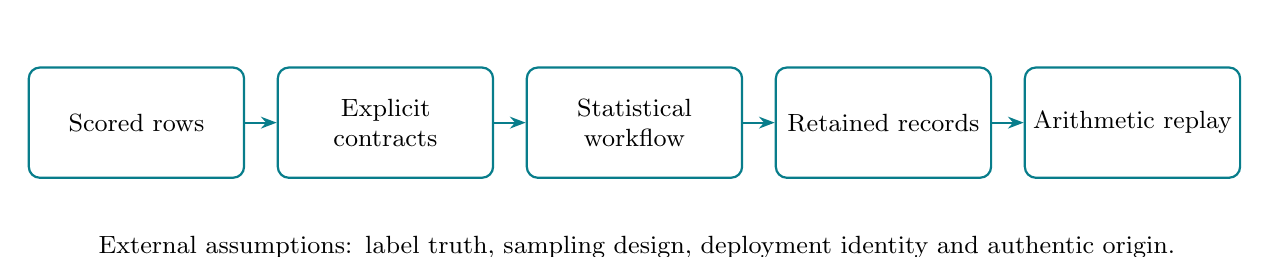
\begin{tikzpicture}[
box/.style={draw=teal,rounded corners,text width=25mm,minimum height=14mm,
align=center,font=\small},
>={Stealth[length=2mm]},every path/.style={draw=teal,thick}]
\node[box] (rows) {Scored rows};
\node[box,right=4mm of rows] (contract) {Explicit contracts};
\node[box,right=4mm of contract] (calc) {Statistical workflow};
\node[box,right=4mm of calc] (record) {Retained records};
\node[box,right=4mm of record] (replay) {Arithmetic replay};
\draw[->] (rows)--(contract);
\draw[->] (contract)--(calc);
\draw[->] (calc)--(record);
\draw[->] (record)--(replay);
\node[below=6mm of calc,align=center,font=\small,text width=140mm]
 {External assumptions: label truth, sampling design, deployment identity and authentic origin.};
\end{tikzpicture}
\caption{Logical layers of the local toolkit, not a deployed multi-tenant
service. Publication correctness and replay do not authenticate external
assumptions.}
\label{fig:architecture}
\end{figure}

\subsection{Different records answer different questions}
Preparation retains an explicit source mapping. Native certification selects an
operating point for a requested budget. A frontier retains a declared grid and
selection evidence. Ordinary rechecks use fresh batches; chains additionally
retain a monitoring horizon and sequence prefix. Release registration instead
freezes an already chosen threshold, criteria, identity and holdout membership.

Local publication distinguishes complete artifacts from interrupted writes and
coordinates chain continuation. Hashes detect changes relative to retained
reference material. They do not supply an external signing authority, trusted
time or proof that no alternate private history exists.

GPU extraction is separate from the ordinary customer path. Fitting and study
code can later use caches or frozen scores. The small customer environment does
not need to load a language model to evaluate an existing scored file.

\section{Data and methods}
\subsection{Recorded question-answer data}
The question source is TriviaQA \citep{joshi2017}. The retained main collection
contains \CorpusRows{} selected questions, partitioned into \TrainRows{}
training, \ValidationRows{} validation and \TestRows{} test rows. The recorded
model is Qwen2.5-7B-Instruct \citep{qwenmodel}, under the manifest's generation
and quantization settings.

The positive label marks a response that fails the project's matching rule.
Lenient alias matching is an operational reference rather than independent
human adjudication. Strict matching supplies sensitivity information, not an
automatically correct replacement.

The last-token feature is the final real prompt position \emph{before}
generation. The classifier standardizes features and fits logistic regression on
training indices; regularization selection uses the declared validation split.
Later project analyses reuse the collection, so not every subsequent use is
described as pristine confirmation.

The model/tokenizer loader does not pass an explicit immutable revision.
Its provenance method records model name and configuration facts rather than a
complete historical weight hash. Model-level reconstruction needs more than a
later download of the same identifier.

\subsection{Constructed transfer and challenge data}
The context-transfer experiment changes prompt context for feature extraction
while reusing the original questions, short-context answers and labels. It
measures representation transfer relative to fixed outcomes, not newly generated
long-context answer accuracy.

The PII studies use authored scenarios, systematic forms and synthetic
identifiers. A companion variant set extends forms beyond the base inventory.
Positive enrichment and shared construction limit transport and independence.

The benign challenge repeats scenarios in different framings. Historical
row-binomial intervals remain replayable but are not current independent-unit
assurance. Selected canaries are regression tripwires, not independent quality
evidence.

\subsection{Quantities and uncertainty}
At a fixed threshold,
\begin{align}
\mathrm{recall}&=\frac{TP}{TP+FN},&
\mathrm{precision}&=\frac{TP}{TP+FP},\\
\mathrm{FPR}&=\frac{FP}{FP+TN},&
\mathrm{flag\ rate}&=\frac{TP+FP}{N}.
\end{align}
AUROC is a positive-versus-negative pair-ranking probability with half credit
for ties. Lift is recall divided by realized flag rate on the same population,
equivalently precision divided by prevalence.

These quantities have different denominators. Precision is undefined when
nothing is flagged; ranking metrics are withheld on a single-class challenge.
Research intervals retain their bootstrap count, seed, grouping and method.
Arithmetic reconstruction does not establish their coverage.

For a fixed rule and independent negative trials, the one-sided exact-binomial
upper bound is
\begin{equation}
U(k,n,\delta)=
\begin{cases}
\mathrm{Beta}^{-1}(1-\delta;k+1,n-k),&k<n,\\
1,&k=n.
\end{cases}
\end{equation}
Selection and dependence require additional arguments.

\subsection{Requested budget and returned number}
Under an appropriate independently fixed scorer and IID calibration design, an
order-statistic procedure can target a fixed-budget proposition
\begin{equation}
\Pr_D\{R(t(D))>B\}\leq\delta.
\label{eq:budget}
\end{equation}
Complete independent review of the implementation/assumption mapping remains
outstanding. The proposition is different from a general claim about a
data-dependent numerical return:
\begin{equation}
\Pr_D\{R(t(D))>U(D)\}\leq\delta.
\label{eq:adaptive}
\end{equation}
Section~\ref{sec:witness} gives a preserved witness against
Equation~\ref{eq:adaptive}, without a violation of Equation~\ref{eq:budget}
in that specified distribution.

Registered release evaluation has a fixed threshold before the holdout.
Its implementation allocates error across five rate intervals and applies the
registered FPR/recall acceptance criteria. The union bound does not require
independence between interval events; each binomial calculation still needs the
appropriate IID design. Grouped release input is unsupported.

\subsection{Independent point audit}
The audit parses every current README-table row, resolves its field uniquely,
checks stated precision and records artifact hashes and source metadata.
A reviewed family registry connects data references, writers, interpretations
and reproduction boundaries.

A separate oracle computes confusion counts and tied-pair AUROC. For each
positive score, binary searches in sorted negative scores count strict wins and
ties. It does not use the original metric-builder formulas to obtain those
points. This is calculation independence, not an independent investigator or
label source.

Missing classifications, invalid score evidence and source changes during
receipt generation are refused. Original scientific artifacts are never
rewritten.

\section{Retained findings}
\subsection{Discrimination and operating trade-offs}
The main held-out AUROC is \claim{C001}, with recorded interval \ci{C001}.
At its operating point, recall is \claim{C002}, precision \claim{C003} and
flag rate \claim{C004} (Table~\ref{tab:operating}).

The independently checked block has \BasePositive{} positive rows among
\BaseRows{} total rows, with \BaseFlagged{} flagged and \BaseTP{} true positives.
High ranking association therefore coexists with many missed positive rows at
that cut. Different targets explain the coexistence arithmetically; AUROC
does not guarantee application usefulness.

\begin{table}[t]
\centering
\caption{The main operating point. Intervals come from retained artifacts;
the point oracle does not independently validate their coverage. Claim IDs
identify the full source ledger.}
\label{tab:operating}
\begin{tabular}{@{}lccc@{}}
\toprule
Quantity&Value&Recorded interval&Claim\\
\midrule
AUROC&\claim{C001}&\ci{C001}&C001\\
Recall&\claim{C002}&\ci{C002}&C002\\
Precision&\claim{C003}&\ci{C003}&C003\\
Flag rate&\claim{C004}&\ci{C004}&C004\\
\bottomrule
\end{tabular}
\end{table}

The broader budget sweep illustrates a trade-off, but its largest-favorable-budget
headline is selected from an observed grid. The validation-selected/test-scored
sweep adds split separation while retaining dirty-source provenance. Neither
creates a fresh external confirmation collection.

\subsection{The pooling rescue did not hold}
In the constructed context transfer, last-token AUROC remains \claim{C029},
mean pooling is near chance at \claim{C030}, and rolling maximum is
\claim{C031} (Table~\ref{tab:transfer}). The latter flags \claim{C032} of
target rows.

\begin{table}[t]
\centering
\caption{Constructed feature transfer. Questions, original responses and labels
are reused; this is not fresh long-context generation accuracy.}
\label{tab:transfer}
\begin{tabular}{@{}lccc@{}}
\toprule
Pooling&Target AUROC&Recorded interval&Claim\\
\midrule
Last token&\claim{C029}&\ci{C029}&C029\\
Mean&\claim{C030}&\ci{C030}&C030\\
Max rolling means&\claim{C031}&\ci{C031}&C031\\
\bottomrule
\end{tabular}
\end{table}

Global averaging may dilute a local feature; maxima over many windows may
emphasize distractor extremes. Position and general feature-distribution changes
are other possible mechanisms. The experiment does not isolate them. The
rolling-window motivation remains a hypothesis that did not establish the
predicted robust alternative.

A stronger mechanism study would predeclare interventions on distractor length,
position and content, keep the source fit fixed, and confirm on independent
questions. That study was not performed.

\subsection{Configuration, planning and monitoring}
Stock PII recall is \claim{C040} and the custom-augmented configuration's recall
is \claim{C044} on the authored challenge. This supports configuration coverage
as important within that inventory. Custom patterns were informed by base
forms, the companion set shares construction choices, and enrichment makes
precision population-specific. Broad superiority to current upstream systems
is not established.

For confirmed positives \(TP\), unflagged volume \(N_u\) and unflagged error
prevalence \(q\), recall on traffic satisfies
\begin{equation}
R(q)=\frac{TP}{TP+qN_u},\qquad
\frac{\partial R}{\partial q}
=-\frac{TPN_u}{(TP+qN_u)^2}.
\end{equation}
The declared workload's derivative is \claim{C056}. Sizing prevalence directly
in recall units targeted the wrong quantity. The retained first-month plan is
\claim{C059} labels under its assumptions; the superseded \claim{C061} remains
failure evidence. Discrete, finite-population and assurance calculations also
matter; the derivative alone is not the headline rule.

Coverage \claim{C063} concerns \claim{C064} simulated trials. No customer
labeling process or commercial saving was measured. Similarly, the year-long
repeated-fixed-test and chained S0 cells report \claim{C066} and
\claim{C067} simulated revocation shares, conditional on their rules and
horizon. The historical capped-monitor cell is not a measurement of the later
repaired runtime.

\subsection{Finite demonstrations and closed extensions}
The gate retains \claim{C086} selected detector-independent comparisons and
blocks \claim{C090} of \claim{C091} authored legitimate workflows. These are
finite-set counts, not production robustness or false-block rates.

The score-free experiment uses conditionally independent simulated votes.
Its results are an optimistic model-specific scenario, not a universal upper
bound for real judges.

The later frozen grader-discovery extension found no new omission under its
bounded method, despite accepted controls. The unscored-trial work closed as a
technical report: strict-cohort agreement is partly an eligibility condition,
and no original execution roster or corrected official ranking is recovered.
Stopping-feedback closed at data feasibility; no policy effect was estimated.
These outcomes remain part of the evidence.

\section{Source audit and assurance limits}
\subsection{Matching values does not reconstruct source}
All \AuditClaims{} numerical rows match their retained fields across
\AuditArtifacts{} artifacts (Table~\ref{tab:audit}). This is not independent
regeneration of every result.

\begin{table}[t]
\centering
\caption{Final source-audit scope, generated from the retained receipt.}
\label{tab:audit}
\begin{tabularx}{\linewidth}{@{}l r X@{}}
\toprule
Check&Count&Meaning\\
\midrule
Matching README rows&\AuditClaims&Agreement at stated precision\\
Result artifacts&\AuditArtifacts&Files directly named by the table\\
Reviewed families&\AuditFamilies&Shared method and source context\\
Dirty-source rows&\DirtyClaims&Producing state not fully identified\\
Frozen-score point targets&\PointTargets&Separate rank/count arithmetic agrees\\
Directly backed README points&\DirectPointClaims&Subset linked to those targets\\
\bottomrule
\end{tabularx}
\end{table}

Dirty-source rows C006--C007, C016--C019 and C020--C028 concern reconciliation,
the out-of-sample sweep and resplit policy results. A dirty flag may reflect an
unrelated untracked file or a substantive edit. Its metadata does not establish
which, so the named commit alone cannot reconstruct the complete original state.

Downstream use requires the same context even when a later writer was clean.
Relabeling an old result under a clean later commit would hide the gap. An
archived original state or a separately identified new study is required.

The point oracle directly backs \DirectPointClaims{} current table claims.
Other rows include counts, statuses, calculations, simulations and measurements
with different reproduction requirements. Standard frozen-score replay also
reconstructs supported intervals using their historical method. That is not
independent interval validation or fresh warrant issuance.

\subsection{Controlled returned-bound counterexample}
\label{sec:witness}
The preserved diagnostic sets \(n=\WitnessN\), \(B=\WitnessBudget\),
\(\delta=\WitnessAlpha\) and design count \(K=\WitnessK\). IID scores in
\(\{0,1,2\}\) have tail probabilities \(q_1=\WitnessQone\) and
\(q_2=\WitnessQtwo\).

Let \(M_1,M_2\) count scores at least 1 and 2. Under the preserved
successor-threshold convention, returned-bound noncoverage is the disjoint union
\begin{equation}
\{M_1\leq1\}\ \cup\ \{M_1\geq2,\ M_2=0\}.
\end{equation}
Its probability is
\begin{equation}
(1-q_2)^n+nq_2(1-q_1)^{n-1}
\approx \WitnessNoncoverage > \WitnessAlpha.
\end{equation}
The exact program enumerates \WitnessStates{} multinomial count states and
checks the closed form with rational arithmetic.

Every selected population risk in this example is \(0,q_1\) or \(q_2\), below
\(B\). The witness challenges the general adaptive returned-U interpretation
without a requested-budget violation in that distribution. It is a known
internal witness reproduced arithmetically, not a new general theorem or a
completed independent production review. FPR-001 remains open.

\subsection{Scope and terminology}
The matrix includes synthetic fixtures and historical method records. A
VALID-cell count is not independently validated model coverage. Historical
dependent-row intervals remain historical despite successful replay.

The vote simulation is likewise an optimistic independent-vote scenario rather
than a universal upper bound. Narrower wording can be scientifically necessary
even when no measured value changes.

\section{Discussion}
The favorable and adverse results have a common implication: evaluation must
retain the proposition that its evidence can actually support. Ranking,
operating recall, future FPR, simulated catch probability and exact workflow
counts cannot share an interpretation merely because they appear together.

A separate calculation can strengthen arithmetic confidence without becoming an
independent experiment. A checksum strengthens byte identity without
authenticating an author. A clean source record improves reproducibility without
proving labels or sampling. An explicit refusal can be a correct outcome.

The supported contribution is a locally executable evaluation instrument and a
research record whose assumptions can be inspected. This report adds an
organized source-connected account of results and limits. Presentation quality
and code volume are not substitutes for novelty, external validation or
production utility.

\section{Threats to validity}
\paragraph{Labels and sampling.}
Alias matching, authored challenges, enrichment and repeated forms limit
interpretation and transport. Independent blinded adjudication was not
completed. Model pretraining exposure to individual questions was not audited.

\paragraph{Selection and reuse.}
Project phases reuse the corpus. Some sweeps are exploratory and some records
have dirty-source provenance. A later declared partition cannot erase earlier
exposure.

\paragraph{Reconstruction.}
Original extraction caches and complete immutable model identity are not all
committed. Score replay is stronger than reading a table but weaker than
reproducing model behavior.

\paragraph{Inference.}
Bootstrap coverage, independent units, conditional nulls and adaptive selection
need their assumptions. FPR-001 and legacy grouped-method limits remain open.
Registered release evaluation has a different design and must not inherit an
unrelated guarantee.

\paragraph{Internal review.}
The oracle is separately implemented arithmetic within the same project, not an
external investigator. Automated assistance was used in implementation and
documentation. Independent human scientific sign-off is not claimed.

\paragraph{Operation.}
No production deployment, authenticated evidence service, buyer study or
commercial benefit is established. Finite demonstrations and simulated years do
not replace those observations.

\section{Reproduction and availability}
The prepared distribution contains the PDF, standalone LaTeX source and a
tracked source/evidence snapshot. Code and third-party notices remain in that
snapshot. Untracked private review material and ignored extraction caches are
excluded.

The development repository was private during preparation. Public reproduction
therefore requires distribution of the accompanying snapshot or access to the
necessary source and inputs. A PDF-only deposit is not a complete reproduction
package. No DOI or publication acceptance is invented by the build.

The main CPU checks are:
\begin{verbatim}
python scripts/verify.py --no-activations
python scripts/audit_documentation.py --links
python -m pytest tests/ -q
\end{verbatim}
New receipts require clean committed source and a new output destination.
Original extraction replay has additional input requirements and is reported
separately; a skipped activation tier is not a pass.

The LaTeX sources use a declared Tectonic toolchain and BibTeX bibliography.
The paper guide records compilation and deposit preparation. Numeric macros are
generated from retained evidence. Typesetting is not a new model experiment.

\section{Conclusion}
Warrant connects local operating decisions to retained evidence and explicit
replay. Its experiments demonstrate useful correlations and important failure
modes. The source audit confirms numerical agreement and separate point
arithmetic, while exposing source gaps and an unresolved guarantee interpretation.
The defensible result is a reproducible, bounded technical artifact with a
transparent account of its limits. Stronger scientific, operational and
publication claims require additional evidence.

\appendix
\section{Evidence map}
The complete per-claim ledger and qualitative register accompany the source.
These families are not one homogeneous experiment.

\begin{longtable}{@{}p{16mm}p{43mm}p{91mm}@{}}
\toprule
Family&Question&Evidence and boundary\\
\midrule
\endhead
F01--F03&Probe and paired comparisons&Validation, reconciliation and paired
artifacts; recorded labels and historical source conditions apply.\\
F04--F06&Budgets and profiles&Exploration and validation/test calculations;
dirty provenance affects the out-of-sample and resplit-policy artifacts.\\
F07--F09&Transfer, drift and matrix&Constructed feature shift and replay;
the inventory includes fixtures.\\
F10--F11&PII and benign challenges&Authored cases and synthetic identifiers;
legacy dependent-row inference is not current assurance.\\
F12--F13&Feasibility and label planning&Declared-scenario arithmetic and
simulation, without production cost measurement.\\
F14--F15&Monitoring&Scenario- and horizon-specific simulations; historical
runtime distinction retained.\\
F16&Label sensitivity&Hypothetical label perturbations; disagreement is
not independent truth.\\
F17&Score-free voting&Conditionally independent simulated votes, not
commercial-judge measurements.\\
F18&Action gate&Finite declared workflows and states, not general
adversarial robustness.\\
\bottomrule
\end{longtable}

\section{Audit and manuscript provenance}
The original consolidated system baseline is
\path{9dbdee03e77b698c497186b9b00297ee506cd0fe}.
The final numerical audit records producing source
\texttt{\AuditSourceCommit}. Its JSON retains selectors, raw hashes,
source flags and explicit exclusions.

Initial and final guarded receipts are both retained. Guard refinements check
source stability and resolve equivalent selectors by object identity rather
than numerical equality. They do not rewrite scientific measurements.

The manuscript source includes metadata, numeric generation, bibliography and
compiler pins. The archival manifest identifies the accompanying source
snapshot. Publishing a Zenodo preprint is a separate author action and does
not imply peer review.

\bibliographystyle{plainnat}
\begingroup\small
\bibliography{references}
\endgroup
\end{document}
